\documentclass{article}
\usepackage[utf8]{inputenc}
\title{Lecture X.Y Topic}
\author{wbg231 }
\date{December 2022}
\newcommand{\R}{$\mathbb{R}$}
\newcommand{\B}{$\beta$}
\newcommand{\A}{$\alpha$}
\newcommand{\D}{\Delta}

\newcommand{\avector}[2]{(#1_2,\ldots,#1_{#2})}
\newcommand{\makedef}[2]{$\textbf{#1}$:#2 }
\usepackage{tikz,graphicx,hyperref,amsmath,amsfonts,amscd,amssymb,bm,cite,epsfig,epsf,url}

\begin{document}

\maketitle

\section{introduction}
\begin{itemize}
\item this is a review of one of the last section of course one, which covers the conditional mean 
\section{conditional mean function }
\item the idea is given random variables a and b. if the value of b is set can we say anything about what we expect the mean of  a to be
\item the conditional mean function of a discrete random variable b given a is $\mu_{b|a}(a)=\Sigma_{b\in B}bp_{b|a}(b|a)$ this is a function of a. it is only defined for values where the conditional distribution of b given a is defined. sometimes written as $E[b|a=a]$
\item for continuous rvs the conditional mean function of b given a is $\mu_{b|a}(a)=\int_{-\infty}^{\infty}bf_{b|a}(b|a)db$ where a is a fixed value that we are conditioning on. 
\item this is a function in that if we set the value of a we get a number out. 
\subsection{example calculation}
\item now as an example for continuous rv consider two random variables a and b with a joint pdf as follows. suppose it represents the  horizontal and vertical position of an otter on a lake.
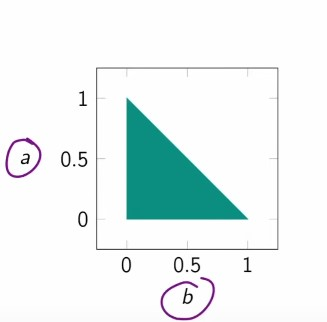
\includegraphics[width=10cm]{notes/averging/review_1.jpg}
\item so our first question is to find the joint pdf. we know it has to be constant on the late meaning that $\int_{0}^{1}\int_{0}^{1-a}cdbda=1$ meaning that c=2 at all points in the triangle and zero otherwise  
\item now suppose we know that the a value of the otter is .85 but we do not know anything about it's b value. so we want the conditional $f(b|a)=\frac{f(b,a)}{f(a)}$ 
\item so we need to solve for the marginal of a, ie $f(a)=\int_{b\in B}f(a,b)=\int_{0}^{1-a}2=2(1-a)$
\item so our conditional can be expressed as $f(b|a)=\frac{f(b,a)}{f(a)}=\frac{2}{2(1-a)}=\frac{1}{1-a} b\in [0,1-a]$ 
\item then we can finally solve for our conditional mean function as $\mu_{b|a}(a)=\int_b bf(b|a) db=\int_{0}^{1-a}b\frac{1}{1-a}db=\int_{b=0}^{b=1-a}\frac{b}{1-a}db=\frac{b^2}{(1-a)2}|_{0}^{1-a}=\frac{(1-a)^2}{2(1-a)}=\frac{1-a}{2}$
\item the point is that the average given we have a is just the point in the middle which makes sense given we have the value of b. 
\item 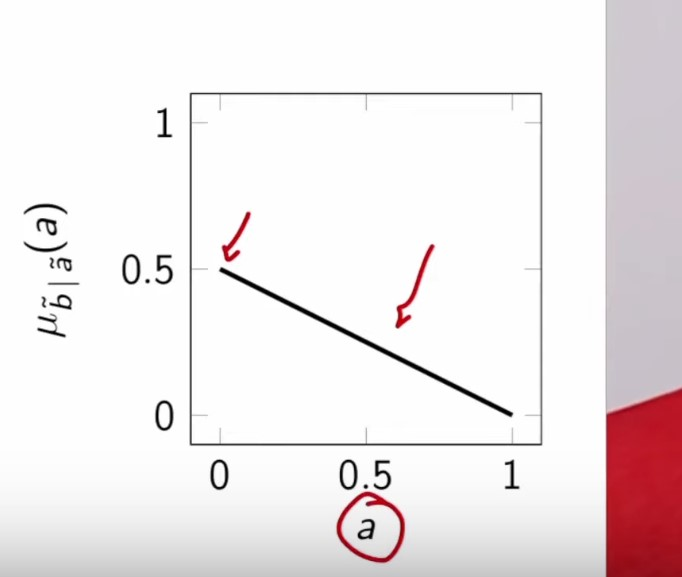
\includegraphics[width=10cm]{notes/averging/review_2.jpg} here we can see that this is a function of a
\section{sample conditional mean for discrete data}
\item suppose we have a data set D=$\{(x_1,y_1)...(x_n,y_n)\}$ where $x_i\in A$ we need tuples so we have joint samples
\item data can be interpreted as samples from some random viable a with range (A)
\item $Y_a=\{y|(a,y)\in D\}$is the set of all tuples with there first entry equal to a (there can be repeated value in this. 
\item $ \hat{m}_{b|a}(a)=\frac{1}{n_a}\Sigma_{y\in Y_a}y
$ where $n_a$ is the number of the entries with first element equal to a, and y is the value of the second entries
\item then we get the mean over this set by taking the averaging of the second entry given the first entry is equal to a. 
\subsection{example}
\item suppose we have the following movie ratings data 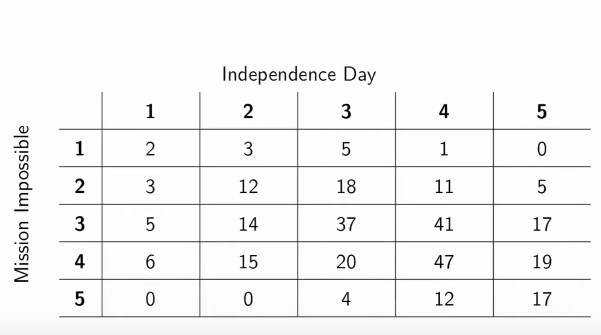
\includegraphics[width=10cm]{notes/averging/review_3.jpg} 
\item each entry is the number of people that rated each movie that number 
\item so what if we want the average rating of mission impossible given Independence day is equal to one? Then we take the average of those values that is $1*\frac{2}{11}+2*\frac{3}{11}+3*\frac{5}{11}+4*\frac{1}{11}$
\item keep in mind again that this is a function of the rating of mission impossible. 
 \section{sample conditional mean for continuous data}
 \item D=$\{(x_1,y_1)...(x_n,y_n)\}$ where $x_i\in A$ we need tuples so we have joint samples
 \item think of the data as coming from random variables a and b 
 \item we can not condition on exact values, so we can either use kde or just use bins 
 \item so for a small $\epsilon$ we can find $Y_{a, \epsilon}=\{y|(x,y)\in D : |x-a|\leq \epsilon \}$ meaning that the value of the first entire is epsilon close to a value of a we set 
 \item the our sample conditional mean is just the average of that set that is $\hat{m}_{b|a}(a)=\frac{1}{n_a}\Sigma_{y\in Y_{a,\epsilon}}y$
\section{iterated expectations motivation}
\item suppose we are int rested in the mean of b, and we have access to the conditional mean function of b given a. 
\item the mean of a random viable is the average of many samples from that random viable
\item so in this  we can think the mean of b as many draws $\{y_1...y_n\}$ from some rv b then $E[b]=\frac{1}{n}\Sigma_{i=1}^{n}y_i$
\item suppose we have some data set D= $\{(x_1,y_1)...(x_n,y_n)\}$ where $x_a\in A$
\item we want to find the mean of b, so we Can def fine bags $Y_{a}=\{y|(a,y)\in D\}$ that is tuples with first entry equal to some value a. 
\item the conditional mean of the second entry given a value of the first entry is our conditional mean function  that is $\mu_{b|a}(a)=\frac{1}{n_a}\Sigma_{y\in y_a}y$ where $n_a$ is the number of elements in $Y_a$
recall also that we can write $P(a=a)=\frac{n_a}{n}$ 
\item so now we want to connect the average of the second entry with the average of the second entry given the value of the first entry. 
\item we we can write $E[b]\approx\frac{1}{n}\Sigma_{i=1}^{n}y_i=\frac{1}{n}\Sigma_{a\in A}\Sigma_{y\in Y_a}y$ where the range of a is A. so we are taking the sum of all the value of the second entries with first entry equal to a for all values of a . 
\item then we can multiply and divide by $n_a$ $\frac{1}{n}\Sigma_{a\in A}\Sigma_{y\in Y_a}y=\Sigma_{a\in A}\frac{n_a}{n}\frac{1}{n_a}\Sigma_{y\in Y_a}y\approx\Sigma_{a\in A}\frac{n_a}{n}\mu_{b|a}(a)\approx \Sigma_{a\in A}P(a=a)\mu_{b|a}(a)\approx E[b]$ in other words the mean of b is a weighted of sum of the conditional mean function 
\item recall that given a random variable a, and a deterministic function h(a) $E[h(a)]=\Sigma_{a\in A}h(a)p(a=a)$ if a is discrete and the sum converges 
\item thus we can really say $E(b)\approx \Sigma_{a\in A}P(a=a)\mu_{b|a}(a)=E[\mu_{b|a}(a)]$ so finding the mean of b is the same as plugging in a and taking the average. 
\item we can see for continuous rv $E(b)\approx \int_{a\in A}f_{a}(a)\mu_{b|a}(a)da$
\section{the conditional mean}
\item the conditional mean function $\mu_{b|a}(a)$ is a deterministic function of a 
\item if we plug in the random variable $\Tilde{a}$ into it we obtain a random variable $\mu_{b|a}(\Tilde{a})$ which we call the conditional mean sometimes writ en as $E[b|a]$ 
\item keep in mind this thing is a random variable. 
\subsection{example}
\item go back to the triangle lake 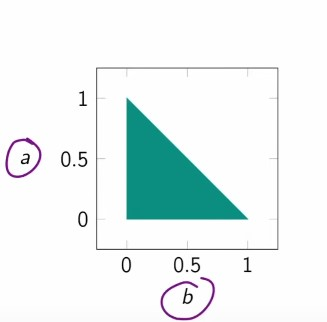
\includegraphics[width=10cm]{notes/averging/review_1.jpg}
\item what is the conditional mean of b given a?
\item we derived earlier that $\mu_{b|a}(a)=\frac{1-a}{2}$
\item so thus we can see that the random variable the conditional mean function is $\mu_{b|a}(\Tilde{a})=\frac{1-\Tilde{a}}{2}$ 
\item so lets look at the distribution of this rv, starting with its cdf $F_{\mu_{b|a}(a)}(x)=P(\mu_{b|a}(a)\leq x)=(\frac{1-\Tilde{a}}{2}\leq x)=P(\Tilde{a}\geq 1-2x$)
\item which can be solved as $\int_{1-2x}^{1}f_{a}(t)dt=\int_{1-2x}^{1}2(1-t)dt=4x^2 for x\in [0,\frac{1}{2}]$ a is only defined between 0 and 1, so x can only be between 0 and one half. 
\item then we can finally get the pdf of our conditional mean function by differentiating the cdf that is $f_{\mu_{b|a}(a)}(x)=8x$
\section{iterated expectations}
\item so we can see that $E{\mu_{b|a}(a)}=\int_{a=\infty}^{\infty}f_{a}(a)\mu_{b|a}(a)da$ then by definition of the conditional mean we can expand this as =$\int_{a=\infty}^{\infty}\int_{b=\infty}^{\infty}f_{a}(a)f_{b|a}(b|a)dbda=\int_{a=\infty}^{\infty}\int_{b=\infty}^{\infty}f_{a,b}(a,b)dbda=E[b]$

so by the example above we can say that $E[\mu_{b|a}(a)]=E[b]$
\item this also work for functions of both a and b, $E[\mu_{h(a,b)|a}(a)]=E[h(a,b)]$
\subsection{example 1 }
\item suppose w have a computer that has t time until it breaks down 
\item suppose that t is is exponential with a parameter set as a function of two other variables o,c that is t=t(h(o,c))=$\frac{1}{o+c}$
\item suppose both o,c uniform in 0,1 
\item and we want to find the mean of t. 
\item given we set o and c we know that t is exponential with parameter $\lambda=\frac{1}{o+c}$
\item thus $\mu_{t|o,c}(o,c)=o+c$ by properties of exponential 
\item then by iterated expectations we can see that $E[t]=E[\mu_{t|o,c}(o,c)]=E[o+c]=E[o]+E[c]=\frac{1}{2}+\frac{1}{2}=1$
\item this is nice because it is simple, and allows us to avoid deriving a complicated density function 
\item watch video 55 in the playlist then the videos on new content .


\section{regression}
\subsection{introduction}
\item suppose we want to predict how an individual rated Independence day given we know how they rated mission impossible 
\item 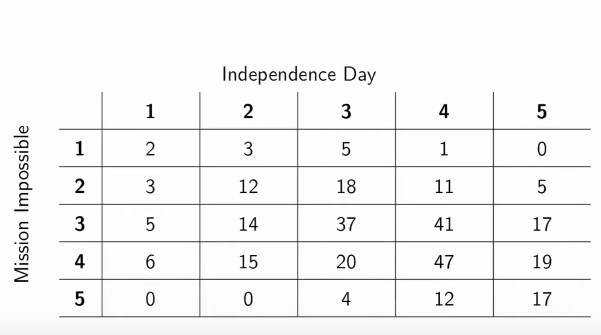
\includegraphics[width=10cm]{notes/averging/review_3.jpg} 
\item we can also do this for continuous random variables.
\item so our goal is to find a function h such that h(a) approximates b when a=a
\item a question is how do we evaluate this estimator? 
\item often with mean squared error that is $mse=E[(b-h(a))^2]=\int_{a\in A}\int_{b\in B} (b-h(a))^2f_{a,b}(a,b)dbda$ that is we are calculating the weighted sum of the square distance between our predicted and observed outcome, weighted by how often we see that outcome  
\item this is averaging the mean squared error in a way that gives more weight to outcomes that occur more 
\subsection{best constant estimator}
\item the best constant estimator of a random variable b is its mean that is $E[b]=argmin_{c \in R}E[(c-b)^1]$
\item so what if we know a=a what value should we chose? the conditional mean of b given a. 
\item recall that the conditional mean function is $\mu_{b|a}(a)$ is a deterministic function of a. ie the average of b given we know the value of a. 
\item this will result in a non linear estimator often times. 
\subsection{conditional expectation estimator}
\item the conditional mean is the min mse estimator 
\item there is a proof for it, but it is kind of tedious.
\subsection{drawbacks}
\item the conditional mean is the minimum mean squared error estimator
\item but it suffers from the curse of dimensionality
\item for higher dimensional data the data requirements we need are exponentially rising. 
\item so we will never find information on the exact quantities we need. 
\item so many more advanced methods for regression are trying to approximate the conditional mean. 
\end{itemize}
\end{document}